
\documentclass[a4paper,12pt]{article}

\usepackage[a4paper, total={6in, 8in}, left=30mm]{geometry}
\usepackage{pdfpages}

\usepackage{cmap}
\usepackage[T2A]{fontenc}
\usepackage[utf8]{inputenc}
\usepackage[english,russian]{babel}
\usepackage{fancyhdr}
\usepackage{minted}
\usepackage{hyperref}
\usepackage{amsmath}

\hypersetup{
  pdfborderstyle={/S/U/W 1}
}

\pagestyle{fancy}
\fancyhf{}
\lhead{Антон Завьялов, ПИ-72}
\rhead{\textbf{Лабораторная №14, вариант 7}}
\cfoot{\thepage}

\makeatletter
\def\@seccntformat#1{%
  \expandafter\ifx\csname c@#1\endcsname\c@section\else
  \csname the#1\endcsname\quad
  \fi}
\makeatother

\begin{document}
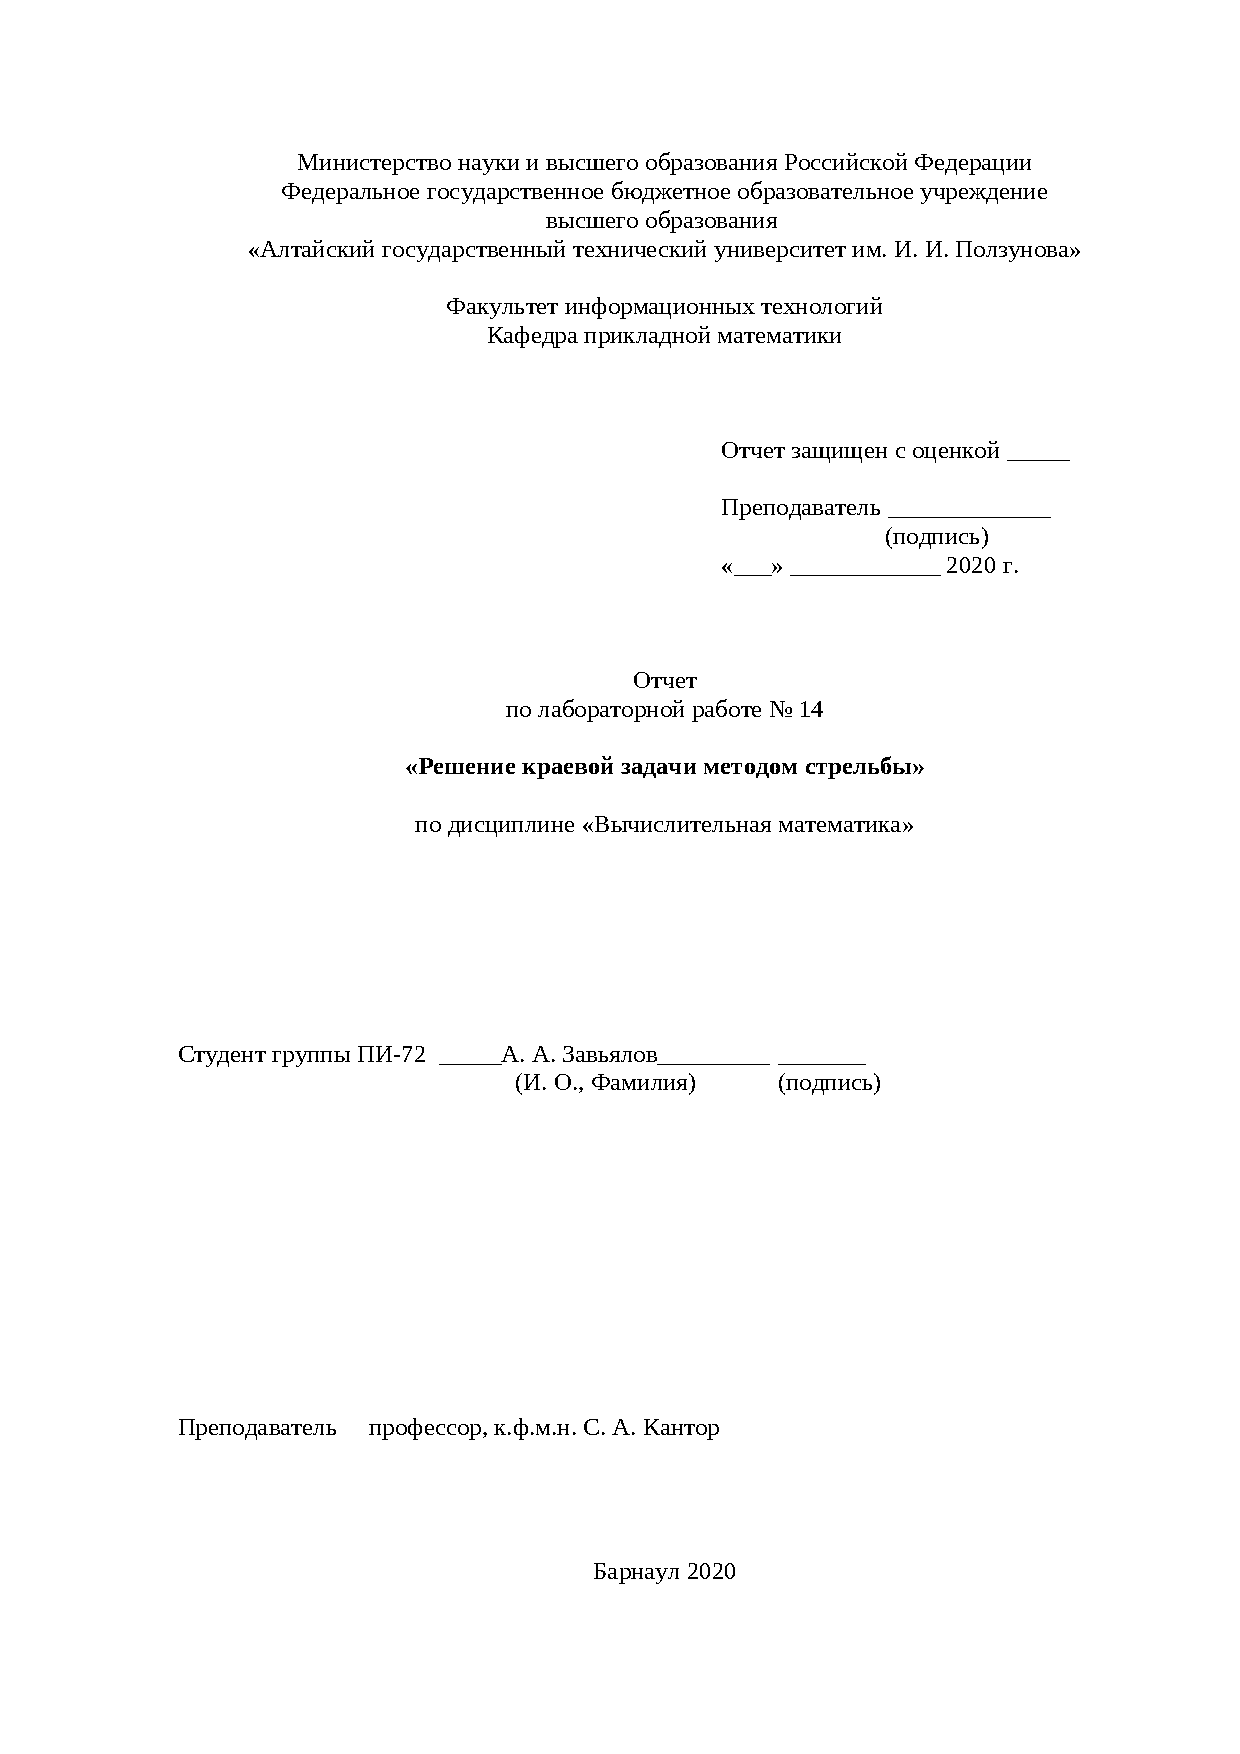
\includepdf[pages={1}]{title.pdf}

\section{\normalsize{Задание к лабораторной работе}}
\begin{flushleft}
    \begin{itemize}
        \item Составить программу решения нелинейной краевой задачи для дифференциального уравнения второго порядка методом стрельбы.
        \item Проанализировать полученный результат, исходя из физического смысла задачи, и при необходимости провести дополнительные вычисления.
    \end{itemize}
\end{flushleft}
\begin{flushleft}
    \textit{Вариант 7.}\linebreak
    Увеличение поверхности тела для выделения тепла в виде излучения имеет большое значение при проектировании сильноточных проводников, так как оно является
    единственным способом отвода излишков тепла. Чтобы масса теплоизлучателя была по возможности наименьшей, его делают в виде набора тонких кольцевых пластин
    с малым углом между боковыми гранями. Распределение температуры в такой пластине является решением уравнения

    \begin{equation}\label{eq:sys}
      \frac{d^2U}{dR^2} + \Bigg(\frac{1}{R + \rho} - \frac{\tg{\alpha}}{(1-R)\tg{\alpha} + \theta}\Bigg)\frac{dU}{dR} - \frac{\beta U^4}{(1-R)\tg{\alpha}+\theta} = 0
    \end{equation}

    с граничными условиями

    \begin{equation}\label{eq:cond}
      U(0) = 1, \frac{dU(1)}{dR} = 0,
    \end{equation}

    где 

    \begin{equation}\label{eq:where}
      R = \frac{r - r_B}{r_T - r_B}, U = \frac{T}{T_B}, \theta = \frac{z_T}{r_T - r_B}, \rho = \frac{z_B}{r_T - r_B}.
    \end{equation}

    Здесь $\alpha$ $-$ угол между гранями пластины; $r, r_B, r_T$ и $z_T$ $-$ текущий радиус, радиус основания, радиус вершины и толщина пластины в вершине соответственно;
    $T$ и $T_B$ $-$ текущая температура и температура основания.\linebreak

    Найти относительную температуру $U$, если $\rho = 0.5$, $\theta = 0.05$, $\alpha = 6^{\circ}$, а $\beta = 0.4$.
\end{flushleft}

\section{\normalsize{Краткое описание метода, расчётные формулы}}
\begin{flushleft}
  \eqref{eq:sys} можно переписать как:

  \begin{equation}\label{eq:sys_same}
    \frac{d^2U}{dR^2} = \frac{\beta U^4}{(1-R)\tg{\alpha}+\theta} - \Bigg(\frac{1}{R + \rho} - \frac{\tg{\alpha}}{(1-R)\tg{\alpha} + \theta}\Bigg)\frac{dU}{dR},
  \end{equation}
  
  тогда

  \begin{equation}\label{eq:sys_sep}
    \frac{dU}{dR} = y,~~\frac{dy}{dR} = \frac{\beta U^4}{(1-R)\tg{\alpha}+\theta} - \Bigg(\frac{1}{R + \rho} - \frac{\tg{\alpha}}{(1-R)\tg{\alpha} + \theta}\Bigg)y,
  \end{equation}

  граничные условия записываются как

  \begin{equation}\label{eq:cond_sep}
    U(0) = 1,~~y(1) = 0.
  \end{equation}

  Запишем недостающее условие как \(y(0) = s\). Подставляя вместо $s$ произвольные значения, получаем возможность решить задачу Коши для \eqref{eq:sys_sep}
  при \(U(0) = 1,~y(0) = s\).\linebreak

  Граничное условие в точке $R=1$ в таком случае зависит от $s$: $y(1,s) = 0$. Найдя $s$, при котором уравнение станет тождеством, найдем решение задачи.
  \linebreak\linebreak
  Найти приближенное значение $s$ можно численно, решая уравнение каким-либо способом (например, методом деления отрезка пополам), причём для каждой итерации
  $y(1,s) = 0$ берётся из решения задачи Коши, тоже решаемой численно (в частности, при помощи метода Рунге-Кутты).
\end{flushleft}


\section{\normalsize{Текст программы с комментариями}}
Кроме расположенных ниже листингов, исходный код можно посмотреть по адресу: \url{https://github.com/andiogenes/differential-equations/tree/master/shooting-method}
\linebreak\linebreak\textbf{Main.hs}
\inputminted[breaklines]{haskell}{../app/Main.hs}

\textbf{Pair.hs}
\inputminted[breaklines]{haskell}{../src/Pair.hs}

\textbf{RungeKutta.hs}
\inputminted[breaklines]{haskell}{../src/RungeKutta.hs}

\textbf{ShootingMethod.hs}
\inputminted[breaklines]{haskell}{../src/ShootingMethod.hs}
\pagebreak
\section{\normalsize{Тестовые примеры}}
\begin{flushleft}
  График решения:\linebreak
\end{flushleft}
\begin{figure}[h]
  \centering
  \def\svgwidth{\columnwidth}
  \input{plot.pdf_tex}
\end{figure}

\end{document}
